\documentclass[11pt, a4paper]{article}

% === PACKAGES ===
\usepackage[utf8]{inputenc}
\usepackage{amsmath}
\usepackage{graphicx}
\usepackage[margin=1in]{geometry} % Standard margin, guide only specifies A4.
\usepackage{setspace}
\usepackage{caption}
\usepackage{tikz}
\usetikzlibrary{shapes.geometric, arrows.meta, positioning, calc}
\usepackage{float}
\usepackage{kotex}

% Page numbers at the bottom center.
\usepackage{fancyhdr}
\pagestyle{fancy}
\fancyhf{} % Clear all header and footer fields
\cfoot{\thepage}
\renewcommand{\headrulewidth}{0pt}
\renewcommand{\footrulewidth}{0pt}

% Double spacing for the main body.
\doublespacing

% Input the TikZ style definitions from your graph.tex file
\tikzset{
    title/.style={font=\Large\bfseries},
    block/.style={rectangle, rounded corners, text width=2.5cm, minimum height=1.5cm, text centered, draw=black, fill=gray!20, font=\small\setstretch{0.9}},
    space/.style={rectangle, rounded corners, minimum width=3.5cm, minimum height=3.5cm, draw=black!80, fill=gray!10, text centered, font=\small\setstretch{0.9}},
    output/.style={diamond, aspect=2, minimum size=1.0cm, text centered, draw=black, fill=gray!20, font=\small\setstretch{0.9}},
    main_arrow/.style={thick, -Triangle, line width=1pt},
    update_arrow/.style={thick, dashed, -Triangle, draw=red!80, rounded corners},
    sarc_emb/.style={circle, fill=red!60, draw=black, minimum size=8pt, inner sep=0pt},
    norm_emb/.style={rectangle, fill=blue!60, draw=black, minimum size=8pt, inner sep=0pt},
    force_arrow/.style={-stealth, dashed}
}

% === DOCUMENT START ===
\begin{document}

% Page numbering for Abstract in lowercase roman.
    \pagenumbering{roman}
    \setcounter{page}{1}

% --- COVER PAGE ---
    \begin{titlepage}
        \centering
        \vspace*{3cm}
        {\huge SimSCLSD: A Simple Framework for Supervised Contrastive Learning of Sarcasm Detection}

        \vspace{1cm}
        {\large 반어 표현 탐지를 위한 단순 지도 대조 학습 프레임워크}
        \vfill

        {\large 2025년 11월}
        \vspace{1.5cm}

        {\large 서울대학교 공과대학} \\
        {\large 전기·정보공학부}

        \vspace{1cm}
        {\large 엄 태 윤}

    \end{titlepage}

% --- APPROVAL PAGE ---
    \begin{titlepage}
        \centering
        \vspace*{2cm}
        {\huge SimSCLSD: A Simple Framework for Supervised Contrastive Learning of Sarcasm Detection}

        \vspace{1cm}
        {\large 반어 표현 탐지를 위한 단순 지도 대조 학습 프레임워크}

        \vfill
        {\large 지도교수 심 규 석}

        \vspace{1cm}
        {\large 이 논문을 공학학사 학위논문으로 제출함}

        \vspace{0.5cm}
        {\large 2025년 11월}

        \vspace{0.5cm}
        {\large 서울대학교 공과대학} \\
        {\large 전기·정보공학부}

        \vspace{0.5cm}
        {\large 엄 태 윤}

        \vspace{1.5cm}
        {\large 엄태윤의 학사 학위논문을 인준함}

        \vspace{0.5cm}
        {\large 2025년 \quad 월 \quad 일}

        \vspace{0.5cm}
        {\large 지도교수 \_\_\_\_\_\_\_\_\_\_ (인)}

    \end{titlepage}

% --- ABSTRACT ---
    \begin{center}
    {\Large\bfseries Abstract}
    \end{center}

    \vspace{1em}
    Detecting sarcasm in online conversational data, such as on Reddit and Twitter, is a significant challenge in Natural Language Processing (NLP). The intended meaning is often the opposite of the literal one and is highly dependent on the surrounding conversational context.
    While pre-trained transformers like BERT and RoBERTa have become standard baselines, they are typically fine-tuned using a Cross-Entropy (CE) loss.
    This approach may not be optimal for learning discriminative representations, especially for a nuanced task like sarcasm where the boundary between classes is subtle.

    Inspired by recent advances in representation learning, we propose a two-stage training framework for sarcasm detection.
    Our model, built on a RoBERTa architecture, first undergoes a "contrastive pre-training" phase on the task-specific dataset.
    This phase utilizes a supervised contrastive loss to learn a more discriminative embedding space.
    The loss function encourages the model to pull representations of same-label examples (e.g., two sarcastic comments) closer together, while simultaneously pushing representations of different-label examples (a sarcastic and a non-sarcastic comment) further apart.
    Following this contrastive phase, the model is fine-tuned using a standard CE loss for the final classification.
    We investigate critical implementation details, such as the use of mean-pooled representations over the standard \texttt{[CLS]} token for the contrastive task.

    We evaluate our approach on the two datasets from the FigLang 2020 Sarcasm Detection shared task: Reddit and Twitter.
    Our experiments demonstrate that this contrastive pre-training step can effectively create more separable representations, showing the potential of supervised contrastive learning as an effective intermediate step for fine-tuning transformers on nuanced classification tasks.

    \vspace{2em}
    \noindent
    \textbf{keywords:} sarcasm detection, supervised contrastive learning, representation learning, text classification, RoBERTa

    \vspace{1em}
    \noindent
    \textbf{Student Number: 2019-18535}

    \clearpage

% --- TABLE OF CONTENTS ---
    \tableofcontents

    \clearpage

% --- MAIN BODY ---
    \pagenumbering{arabic}
    \setcounter{page}{1}


    \section{Related Work}
    Our research is positioned at the intersection of three key areas: \textbf{(1)} sarcasm detection as a context-dependent task, \textbf{(2)} the use of Transformer-based models for this task, and \textbf{(3)} the application of supervised contrastive learning to improve representation quality in NLP.

    \subsection{Sarcasm Detection and Context}
    Sarcasm detection is typically framed as a binary classification task (sarcastic vs. non-sarcastic).
    It is a critical sub-problem in NLP, as accurately identifying sarcastic intent is essential for understanding a user's true sentiments and beliefs.
    The primary challenge is that sarcastic utterances often use positive words to convey a negative meaning, making the literal text misleading.

    Researchers have shown that for both humans and computers, \textbf{conversational context is vital} for correctly identifying sarcasm.
    An isolated response like ``Man, I've seen more than that on a Friday night!'' is ambiguous, but it becomes clearly sarcastic when preceded by the context ``People think 5 tonnes is not a lot of cocaine''.
    The FigLang 2020 shared task \cite{ghosh2020report}, the source of our datasets, was specifically designed to benchmark models on their ability to leverage this conversational context.

    \subsection{Transformer Models for Sarcasm Detection}
    While early approaches relied on feature-based machine learning models, the field is now dominated by pre-trained Transformer architectures.
    A review of the FigLang 2020 task \cite{ghosh2020report} shows that nearly all top-performing systems used variants of BERT \cite{devlin2019bert} and RoBERTa \cite{liu2019roberta}.

    A key design choice for these models is how to present the conversational context to the model.
    \begin{itemize}
        \item \textbf{Concatenation:} The most common approach is to simply concatenate the context and the target response into a single input sequence.
        \item \textbf{Hierarchical Models:} More complex methods, such as that by Srivastava et al. (2020) \cite{srivastava2020novel}, use a hierarchical architecture.
        They first encode all context sentences, pass them through a summarization (e.g., CNN and LSTM) layer, and then combine this summarized context representation with the response representation for a final prediction.
        \item \textbf{Context Separators:} Pant and Dadu (2020) \cite{pant2020sarcasm}, in their work on the same dataset, demonstrated that explicitly formatting the input matters.
        They found that fine-tuning RoBERTa with a special \texttt{<context\_sep>} token between the context and the response yielded a \textbf{5.13\% F1-score improvement} on the Reddit dataset compared to simple concatenation \cite{pant2020sarcasm}, highlighting that the model can learn the significance of this structural boundary.
        Our work adopts this separator-based input format.
    \end{itemize}

    \subsection{Supervised Contrastive Learning for NLP}
    The vast majority of Transformer-based classifiers are fine-tuned using a standard \textbf{Cross-Entropy (CE) loss}.
    However, CE has known limitations; it optimizes for correct classification but does not explicitly enforce a discriminative embedding space.
    This can lead to poor margins and instability, especially on noisy or nuanced datasets.

    \textbf{Contrastive Learning} has emerged as a powerful alternative for representation learning.
    It was popularized in self-supervised vision (e.g., SimCLR), where the goal is to "pull" representations of augmented views of the same image (positives) together while "pushing" representations of all other images (negatives) apart.

    Our work uses \textbf{Supervised Contrastive (SupCon) Learning}, an extension formalized by Khosla et al. (2020) \cite{khosla2020supervised} that leverages label information.
    Instead of only pulling augmented views of one sample together, the SupCon loss aims to pull all samples belonging to the \textbf{same class} into a tight cluster in the embedding space, while simultaneously pushing apart clusters of samples from different classes.
    This approach has been shown to create more compact and well-separated clusters than CE for text classification.

    This technique has been successfully applied as an intermediate training step for large language models.
    Works like Li et al. (2021) \cite{li2021simclad} and Moukafih et al. (2022) \cite{moukafih2022simscl} have proposed ``continual contrastive pre-training'' or ``simple supervised contrastive'' frameworks to adapt a general-purpose model (like BERT) to a specific task's feature distribution \textit{before} the final classification fine-tuning.

    Our work builds on these ideas, proposing a two-stage approach that first uses the SupCon loss to adapt a RoBERTa model to the sarcastic vs. non-sarcastic feature space, before fine-tuning with a standard CE loss for the final classification.

    \section{Proposed Method}
    Our approach is a two-stage framework that first adapts a pre-trained RoBERTa model to the sarcasm task using supervised contrastive learning, and then fine-tunes this adapted model for final classification. This method is designed to create a more discriminative and well-separated embedding space before the final classification, which is particularly useful for a nuanced task like sarcasm detection.

    The two stages, as illustrated in Figure \ref{fig:stage1} and Figure \ref{fig:stage2}, are:
    \begin{enumerate}
        \item \textbf{Stage 1: Supervised Contrastive Pre-training:} The model's encoder is trained using a supervised contrastive loss.
        This stage teaches the model to pull representations of samples with the same label (e.g., two sarcastic comments) closer together in the embedding space, while simultaneously pushing samples with different labels (one sarcastic, one not) apart.
        \item \textbf{Stage 2: Classification Fine-tuning:} The contrastively-trained encoder's weights are used as the starting point.
        A new classification head is added, and the entire model is fine-tuned on the same dataset using a standard Cross-Entropy loss.
    \end{enumerate}

    \begin{figure}[H]
        \centering
        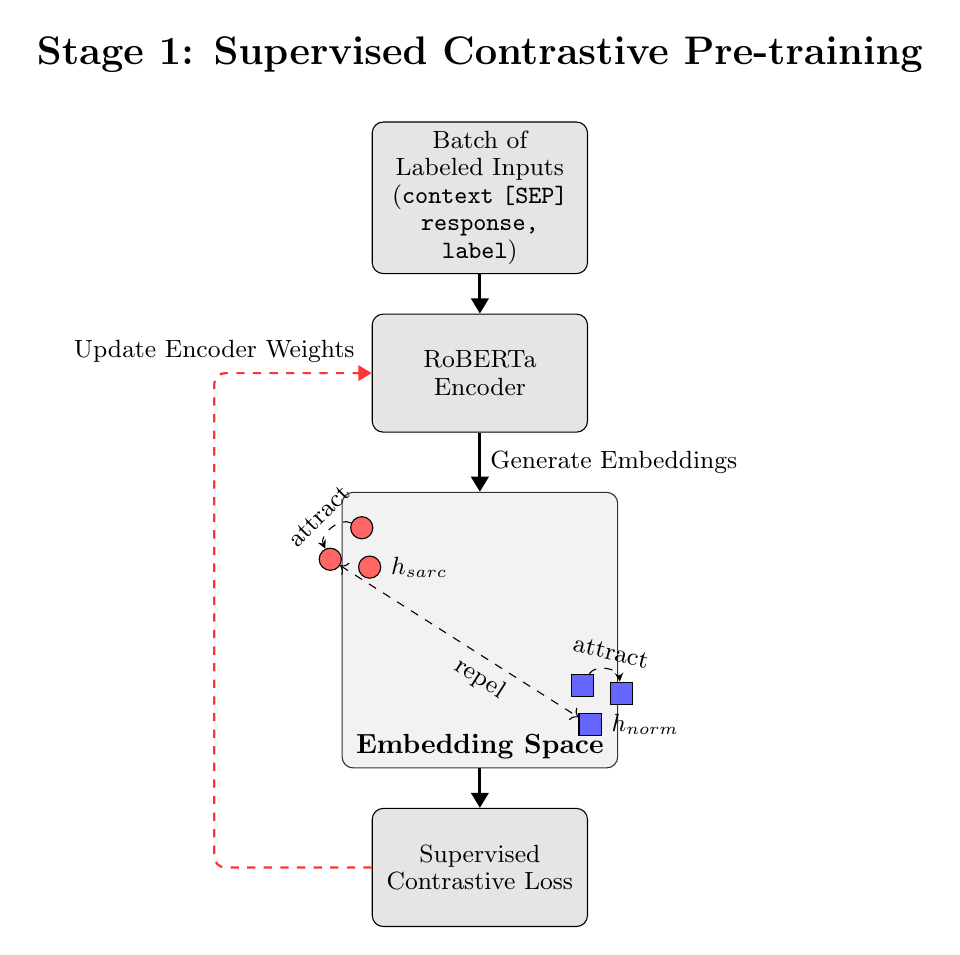
\begin{tikzpicture}[node distance=.5cm]

    % --- Title ---
    \node (title) [title] {Stage 1: Supervised Contrastive Pre-training};

    % --- Input Data ---
    \node (input) [block, below=of title] {Batch of Labeled Inputs \\ \small(\texttt{context [SEP] response, label})};

    % --- RoBERTa Encoder ---
    \node (encoder) [block, below=of input] {RoBERTa Encoder};
    \draw [main_arrow] (input) -- (encoder);

    % --- Embedding Space ---
    \node (emb_space) [space, below=.75cm of encoder] {};
    \node [above] at (emb_space.south) {\textbf{Embedding Space}};
    \draw [main_arrow] (encoder) -- (emb_space) node [midway, right, font=\small] {Generate Embeddings};

    % Coordinates for embedding clusters
    \coordinate (c1) at ($(emb_space.center)+(-1.5, 1.3)$); % Sarcastic cluster
    \coordinate (c2) at ($(emb_space.center)+(1.3, -0.7)$); % Not Sarcastic cluster

    % Sarcastic Embeddings (Circles)
    \node[sarc_emb] (s1) at (c1) {};
    \node[sarc_emb] (s2) at ($(c1)+(-0.4,-0.4)$) {};
    \node[sarc_emb, label={[font=\small]right:$h_{sarc}$}] (s3) at ($(c1)+(0.1,-0.5)$) {};

    % Not Sarcastic Embeddings (Squares)
    \node[norm_emb] (n1) at (c2) {};
    \node[norm_emb] (n2) at ($(c2)+(0.5,-0.1)$) {};
    \node[norm_emb, label={[font=\small]right:$h_{norm}$}] (n3) at ($(c2)+(0.1,-0.5)$) {};

    % Force arrows illustrating the contrastive objective
    \draw[force_arrow, black, bend right=70] (s1) to node[midway, above, sloped, font=\small] {attract} (s2);
    \draw[force_arrow, black, bend left=70] (n1) to node[midway, above, sloped, font=\small] {attract} (n2);
    \draw[force_arrow, black, <->] (s2) to node[midway, below right, sloped, font=\small] {repel} (n3);

    % --- Loss Function ---
    \node (loss) [block, below=of emb_space] {Supervised Contrastive Loss};
    \draw [main_arrow] (emb_space) -- (loss);

    % --- Weight Update Path ---
    \draw [update_arrow] (loss.west) -- ++(-2,0) |- (encoder.west)
    node [midway, above, font=\small] {Update Encoder Weights};

\end{tikzpicture}
        \caption{Stage 1: Supervised Contrastive Pre-training. The encoder learns to map same-label inputs into nearby clusters and different-label inputs into distant clusters.}
        \label{fig:stage1}
    \end{figure}

    \begin{figure}[H]
        \centering
        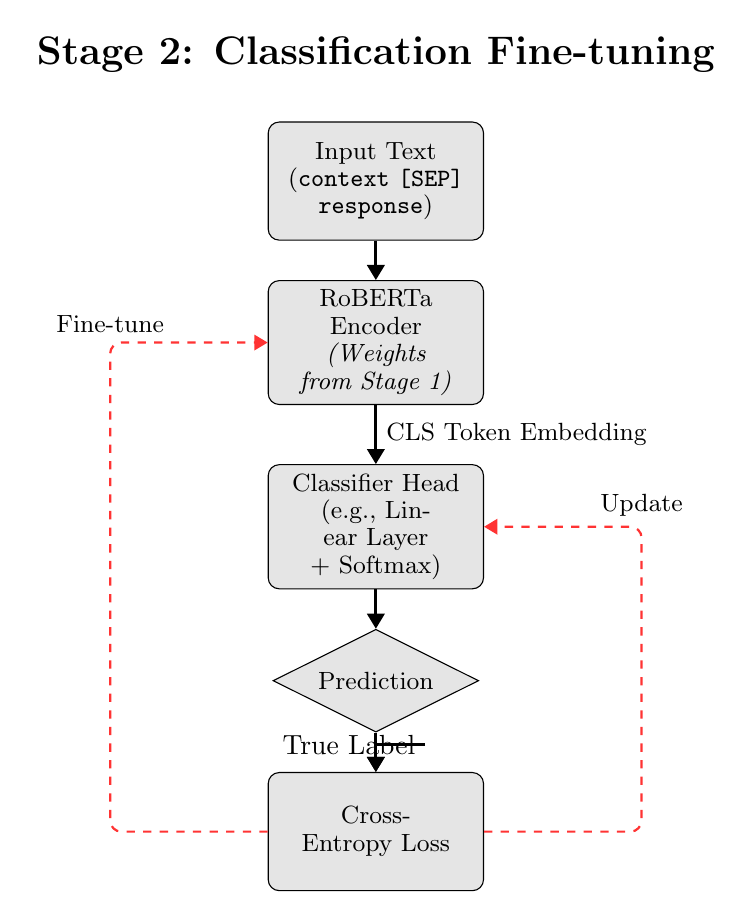
\begin{tikzpicture}[node distance=.5cm]

    % --- Title ---
    \node (title) [font=\Large\bfseries] {Stage 2: Classification Fine-tuning};

    % --- Input Data ---
    \node (input) [block, below=of title] {Input Text \\ \small(\texttt{context [SEP] response})};

    % --- RoBERTa Encoder ---
    \node (encoder) [block, below=of input] {RoBERTa Encoder \\ \small\textit{(Weights from Stage 1)}};
    \draw [main_arrow] (input) -- (encoder);

    % --- Classifier Head ---
    \node (classifier) [block, below=.75cm of encoder] {Classifier Head \\ \small(e.g., Linear Layer + Softmax)};
    \draw [main_arrow] (encoder) -- (classifier) node [midway, right, font=\small] {CLS Token Embedding};

    % --- Final Prediction ---
    \node (prediction) [output, below=of classifier] {Prediction};
    \draw [main_arrow] (classifier) -- (prediction);

    % --- Loss Calculation (Revised Style) ---
    \node (loss) [block, below=of prediction] {Cross-Entropy Loss};
    \draw [main_arrow] (prediction) -- (loss);

    % Replace the block with a simple text node for the label
    \node (label_text) [above left=0.1cm and -2cm of loss] {True Label};
    \draw [main_arrow] (label_text) -| (loss.north);

    % --- Weight Update Paths ---
    % Path to update the classifier (rerouted to the right)
    \draw [update_arrow] (loss.east) -- ++(2,0) |- (classifier.east)
    node [midway, above, font=\small] {Update};

    % Path to update the main encoder (originating from a clean point)
    \draw [update_arrow] (loss.west) -- ++(-2,0) |- (encoder.west)
    node [midway, above, font=\small] {Fine-tune};

\end{tikzpicture}
        \caption{Stage 2: Classification Fine-tuning. The adapted encoder from Stage 1 is used as a base, and a new classifier head is trained with a standard Cross-Entropy loss.}
        \label{fig:stage2}
    \end{figure}

    \subsection{Model Architecture and Input}
    Our base model is \textbf{RoBERTa-base} \cite{liu2019roberta}, which we load using the \texttt{AutoModel} class from the Hugging Face \texttt{transformers} library.

    For both training stages, we format the input by concatenating the conversational context with the target response, following the findings of the FigLang 2020 shared task \cite{ghosh2020report}.
    As shown in our \texttt{dataset.py} code, all context turns are joined by a \texttt{[SEP]} token, and another \texttt{[SEP]} token is used to separate the full context from the target response.
    This creates a single input sequence formatted as:
    \begin{center}
        \texttt{[CLS] context\_1 [SEP] context\_2 [SEP] ... [SEP] target\_response [EOS]}
    \end{center}

    \subsection{Stage 1: Supervised Contrastive Pre-training}
    The goal of this stage is to learn a high-quality representation $z$ for each input.
    In our implementation, we use the embedding of the \texttt{[CLS]} token as the representation for the entire sequence.
    This representation $z_i$ (the \texttt{[CLS]} token's hidden state for sample $i$) is then fed into the supervised contrastive loss function.

    This loss function, which we implement in \texttt{loss.py}, is based on the $\mathcal{L}_{\text{out}}^{\text{sup}}$ formulation from Khosla et al. (2020) \cite{khosla2020supervised}.
    The loss for a batch of $N$ samples is defined as:

    $$
    \mathcal{L}_{\text{SupCon}} = \sum_{i \in I} \frac{-1}{|P(i)|} \sum_{p \in P(i)} \log \frac{\exp(z_i \cdot z_p / \tau)}{\sum_{a \in A(i)} \exp(z_i \cdot z_a / \tau)}
    $$

    Where:
    \begin{itemize}
        \item $i \in I \equiv \{1 \dots N\}$ is the index of an ``anchor'' sample in the batch.
        \item $z_i$ is the normalized \texttt{[CLS]} embedding of the anchor sample $i$.
        \item $P(i) \equiv \{p \in A(i) : y_p = y_i\}$ is the set of all other samples in the batch (positives) that have the \textbf{same label} as the anchor $i$.
        \item $A(i) \equiv I \setminus \{i\}$ is the set of all samples in the batch other than the anchor $i$.
        \item $\tau$ is a scalar temperature hyperparameter, which we set to \texttt{0.07} in our configuration.
    \end{itemize}

    During this stage, the entire model (RoBERTa encoder and projection head) is trained for 3 epochs with an AdamW optimizer and a learning rate of $1 \times 10^{-5}$.

    \subsection{Stage 2: Classification Fine-tuning}
    After the contrastive pre-training is complete, the model's encoder weights are saved.
    We then begin Stage 2, which is a standard classification fine-tuning process.

    The \texttt{SarcasmModel} is loaded with the weights from Stage 1. The \texttt{forward} pass for this stage (when \texttt{is\_pretraining=False}) takes the \texttt{[CLS]} token's embedding, passes it through a dropout layer, and then feeds it into the final linear classification layer to produce logits.

    These logits are passed to a \textbf{Cross-Entropy Loss} function. A key implementation detail is the use of \textbf{differential learning rates}.
    The optimizer is re-initialized to train the pre-trained RoBERTa base model (\texttt{model.model}) with a very low learning rate of $1 \times 10^{-6}$, while the newly added classifier head (\texttt{model.classifier}) is trained with a higher learning rate of $1 \times 10^{-5}$.
    This allows the classifier to learn quickly without causing catastrophic forgetting in the extensively trained encoder.
    This stage is also run for 3 epochs.

% --- REFERENCES ---
    \bibliographystyle{IEEEtran}
    \bibliography{references}

\end{document}



